% Appendix A
\label{AppendixA-methods} % For referencing this appendix elsewhere, use \ref{AppendixA}
\chapter{Methods} % Main appendix title

Procedures used to set up experiments are detailed in this appendix.

\section{Cleaning data}

Data corruption was found with Unity3D generated datasets where some .json files were not generated, leading to missing steering angles and throttle values for some images. There "orphaned" images were deleted with script src/utils/jsonclean.py

\section{Running the car simulator}
\label{RunningCarSimulatorForInference}

The main testing environment consisted of a Dell Precision Tower 5810 with a 6 core Intel Xeon Processor and 32GB memory running Ubuntu 18.04. Unity Hub 2.3.2 was installed then run as sudo:
\begin{verbatim}
$ sudo ./UnityHub.AppImage --no-sandbox 
\end{verbatim}
The car simulator source was cloned from:
\begin{verbatim}
$ git clone https://github.com/dsikar/sdsandbox.git    
\end{verbatim}
The Unity project contained in sdsandbox/sdsim can then added and loaded.
Once the menu scene runs, one of 5 circuits can be chosen. Once the chosen circuit is loaded, there are options to \textit{Auto Drive w Rec} (generate test data and steering angle using PID control) or \textit{NN Control over Network} (send images over network and receive predicted steering angles). The first case will output files to ../output directory, the second case will send and listen to network messages. The handshake process has been captured with tcpflow and stored to  src/debug/tcpflow\_output.txt. The prediction engine starts returning predicted steering angles after the 4th frame sent by simulator as described in section \ref{NetMonDebug}

\begin{figure}[ht]
 \centering 
 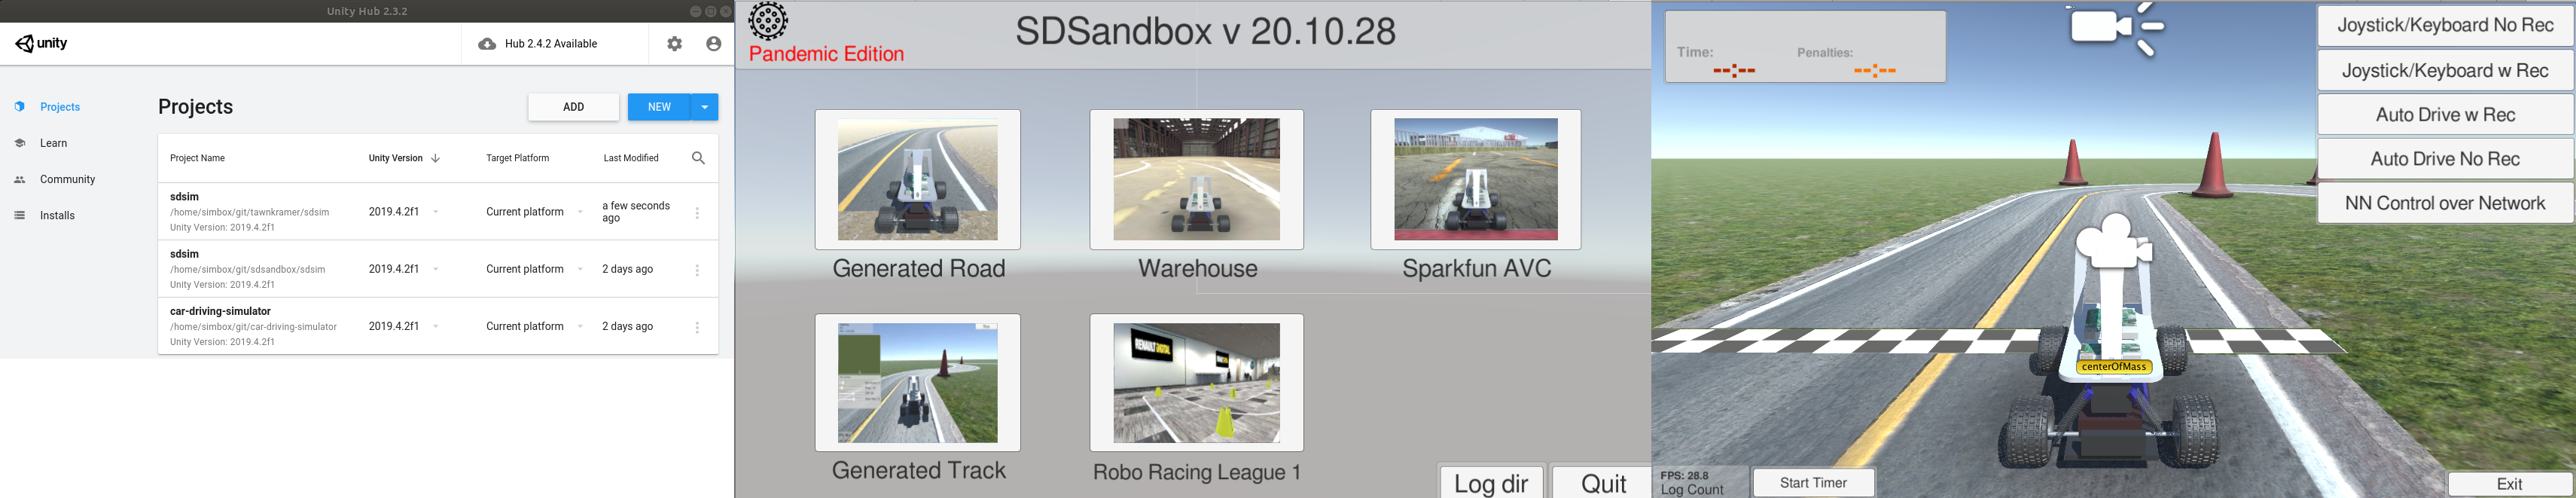
\includegraphics[scale=0.17]{Figures/UnityHubSDSandbox3in1.png}
 \caption{Left to right: Unity Hub, SDSandbox home screen and simulation ready to run}
 \label{fig:SDSandboxHome}
\end{figure}



\section{Network monitoring and debugging}
\label{NetMonDebug}
tcpflow (\cite{garfinkel2013passive}) was used to monitor network traffic between car simulator and neural network prediction engine. Once the simulator is setup to run in neural network mode and before the predict\_client.py prediction engine starts, tcpflow is launched set to listen on the loopback interface port 9091, and output network traffic packets to console:
\begin{verbatim}
$ sudo tcpflow -i lo -c port 9091
\end{verbatim}
The prediction script then runs, and JSON (\cite{pezoa2016foundations}) a lightweight data-interchange format, tcp packets may be monitored and debugged. Simulator packets are distinguished by \textit{telemetry} and prediction engine packets by \textit{control} msg\_types respectively, as shown in excerpt:
\begin{verbatim}
127. (...) {"msg_type":"telemetry",(...),"image":(...)
127. (...) {"msg_type": "control", "steering": "-0.09476048" (...)
\end{verbatim}
The packets carry the image sent from sim to prediction engine, and returned steering angle prediction.

\section{Generating Plots}

This section describe the tools used to generate plots.

\subsection{Steering angle comparison}

Plots were generated with Jupyter Notebook:
\begin{verbatim}
    src/utils/
\end{verbatim}

\section{Datasets}

A template directory structure was created such that downloaded data could be accessed in code with the same paths. The structure exists in the datasets repository and once cloned creates the template directory:
\begin{verbatim}
$ git clone https://github.com/dsikar/msc-data
$ tree -d msc-data/
msc-data/
 audi
 ford
 kitti
 mechanical-turk
 udacity
 unity
\end{verbatim}

\subsection{Ford AV Dataset}

The steering angles can be extracted from .bag files using ROS commands:
\begin{verbatim}
    # In one terminal, start ros engine
    $ roscore
    # In another terminal, inspect content of bag file
    $ time rosbag info Sample-Data.bag
    (...)
             /imu                 146939 msgs    : sensor_msgs/Imu             
    (...)
             /pose_ground_truth   146136 msgs    : geometry_msgs/PoseStamped   
             /pose_localized       16100 msgs    : geometry_msgs/PoseStamped   
             /pose_raw            146190 msgs    : geometry_msgs/PoseStamped   
(...)
    # And subscribe to topic of interest 
    $ rostopic echo /imu | tee sample_imu.yaml
    # In another terminal, playback bag file
    $ time rosbag play --immediate Sample-Data.bag --topics /imu
    # Sanity check, count number of acquisitions
    $ cat sample_imu.yaml | grep "orientation:" | wc -l
\end{verbatim}
The snippet above generates file imu.yaml, with all pose data generated by imu device. From this file we extract the steering angle, which is the z axis (yaw) of the orientation field (TODO check .yaml dialect). 
Images can be extracted from the same bag file with the Python 2.7 bag\_to\_images.py script:
\begin{verbatim}
    $ python2 bag_to_images.py Sample-Data.bag ~/git/msc-data/ford/sample/ros/ \
        /image_front_left
\end{verbatim}
Each image is an attribute in a dictionary, which also contains seconds (secs) and nano seconds (nsecs) attributes within the header attribute:
\begin{verbatim}
header: 
  seq: 213414
  stamp: 
    secs: 1501822147
    nsecs: 684951066
  frame_id: "camera_front_left"
height: 215
width: 414
encoding: "8UC3"
is_bigendian: 0
(...)
\end{verbatim}
Thus a timestamp can be obtained for each image extracted. This is done with script parse\_yaml\_time.py:
\begin{verbatim}
    
\end{verbatim}
While the steering angles are extracted 
The image can be matched with a steering angle by obtaining the timestamp of image, the full secs 

\section{Automold}
The rainy images were created with:  
\begin{verbatim}
github.com/dsikar/automold/RainyImagesDissertationPlot.ipynb
\end{verbatim}

\section{Development Environments}

\subsection{Intel DevCloud}

Intel provides a 200GB storage quota. Storage use can be checked with getquota command:
\begin{verbatim}
$ getquota
199.78 GB out of 200.00 GB (99.89%) used   
\end{verbatim}
Jobs are queued with qsub command:
\begin{verbatim}
    $ qsub -l nodes=1:gpu:ppn=2 ford_sample_download.sh -l walltime=23:59:59
\end{verbatim}
where the actual commands that run e.g. downloading data, training and testing networks are scripted in a batch file e.g. ford\_sample\_download.sh, train.sh.   
The queue can be checked with watch command:
\begin{verbatim}
    $ watch -n 1 qstat
\end{verbatim}
Jobs can run for a maximum of 24 hours, any job exceeding that execution time is terminated automatically. Jobs can be deleted from queue with qdel command.

\section{Tensorflow and Keras}
\label{methods:tensorflow-keras}
The versions used were 2.2.0 and 2.4.3 respectively. To ensure the same versions are installed in all development platforms, run:
\begin{verbatim}
$ pip install keras --user
$ pip install tensorflow --user
# to check versions
$ python3
>>> import keras
>>> keras.__version__
'2.4.3'
>>> import tensorflow
>>> tensorflow.__version__
'2.2.0'
\end{verbatim}
If the modules are already present in the environment, but a lower (earlier) version e.g.:
\begin{verbatim}
>>> tensorflow.__version__
'1.15.4'    
\end{verbatim}
it can be upgraded by running:
\begin{verbatim}
$ pip install --ignore-installed --upgrade tensorflow==2.2.0 --user
\end{verbatim}

\subsection{Recording one loop around a track}

To record the images and steering angles generated by going around a track once, on the terminal:
\begin{verbatim}
$ sudo ./UnityAppimage --no-sandbox
\end{verbatim}
Open the project in sdsim directory (commit ed0cc0b)

\subsection{Running simulator predictions}
\label{running-simulator-predictions}

To run predictions, and to monitor TCP traffic:
\begin{verbatim}
# Run unity from one terminal run:
$ sudo ./Unity.AppImage --no-sandbox
# To monitor TCP traffic, from another terminal run:
$ sudo tcpflow -i lo -c port 9091 > /tmp/tcpflow.log
# To run predictions, from another terminal run:
$ python predict_client.py \
--model=../trained_models/nvidia_baseline/20201120124421\_nvidia\_baseline.h5
\end{verbatim}

% there probably will not be enough time to use ROS at scale so parking this for now in appendix, might leave for future reference or remove
\section{ROS}
The Robot Operating System (\cite{quigley2009ros}) is middleware, that is, placed between the operating system an the application program. It helps manage complexity and distributed systems, such as a managing the process of recording several sensor outputs in a moving vehicle. The term "plumbing" is sometimes used, as parts of a distributed application are connection with "data pipes".  
ROS was used to store data from the FORD AV dataset.

% \section{Extracting steering angles with ROS}
Info on how to get a steering angle (YAW) using quaternions and the IMU data.

